\documentclass[a4paper,10pt]{article}
\usepackage{graphicx}

\textheight=25.5cm
\textwidth=17.5cm
\voffset=0.cm
\hoffset=-0.0cm
\oddsidemargin -1cm
\evensidemargin -1cm
\topmargin -2cm
\baselineskip=0.900cm
\setlength{\parindent}{0in}

\graphicspath{{figures/}}

\begin{document}

\subsection{Overlap with 4MOST extragalactic surveys}

Authors: I.Hook, J. Carrick, R. Biswas.

\vspace{0.2cm}

The 4MOST facility will be a highly multiplexed, optical, fibre-fed
spectrograph mounted on the 4-metre VISTA telescope. It is due to
start operations at the end of 2022. Its wide field of view (4.1 sq
deg), high multiplex (1600 fibres feeding low-resolution spectrographs
suitable for extragalactic science plus $\sim 800$ fibres feeding a
high-resolution spectrograph, primarily for galactic science) and
geographical location (near the Paranal site in Chile) makes 4MOST an
ideal spectroscopic follow-up facility for LSST. The scientific
synergy potentially covers a very wide variety of science goals. Here
we focus on the synergy for follow-up of transients and varying
sources.

The 4MOST-TiDES survey plans to piggy-back on other 4MOST
extragalactic surveys, and will use a small subset of the fibres in
each pointing to observe live transients and the host galaxies of
previously-discovered transients. The 4MOST extragalactic surveys will
be carried out over a large fraction of the southern sky, shown in
Figure~\ref{4most_sky}.  There is also a component of TiDES that aims
to obtain spectral time-sequences of AGN in 4MOST's deep fields (that
are likely to coincide with at least a subset of LSST's deep fields,
TBD), for reverberation mapping.


\begin{figure}[hc]
\begin{centering}
  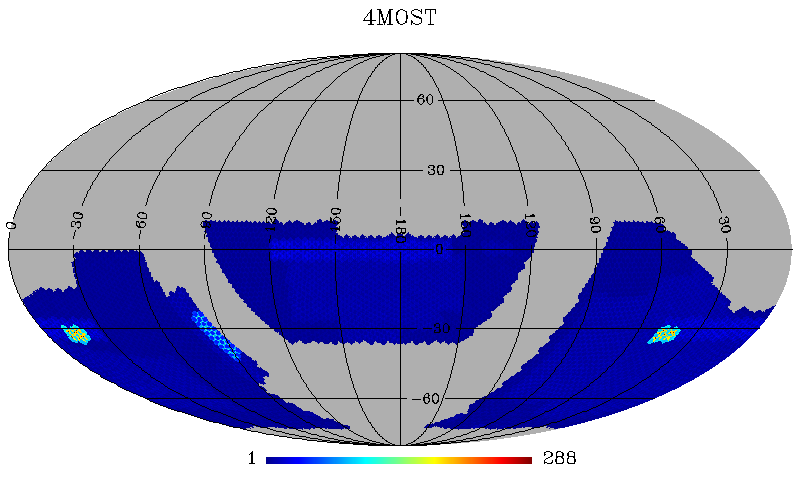
\includegraphics[width=10.0cm]{4most_fndep.png}
\end{centering}

\caption{One realisation of the sky coverage of 4MOST extragalactic
  surveys, colour coded by number of visits. This is based on
  4MOST-4FS survey simulation round9/c/run01 dated 2018-5-14. Note
  that the 4MOST survey design is still in progress and the map is
  likely to change.}
\label{4most_sky}
\end{figure}

There is a preference for 4MOST to observe within the approximate
declination range seen in Figure~\ref{4most_sky} for several
reasons. One is not to duplicate other facilities in the North (such
as DESI, Subaru-PFS and WEAVE). Another is that the winds from the
north at Paranal can make it difficult to observe in that
direction. Similarly, 4MOST prefers not to observe far South because
of inefficiency when observing at high airmass. The 4MOST Atmospheric
Dispersion Compensator works optimally upto zenith distances of 55
degrees, equivalent to airmass of $\sim1.75$. At larger airmasses,
light is lost at the ends of the spectrum. Because VISTA is at
latitude $\sim -24.7$ degrees, one can therefore observe theoretically
to declination of $\sim -80$ degrees at the meridian. In practice
4MOST will not go much below declination of $-70$ degrees, except in
the Magellanic Clouds, as observations get much harder to schedule if
one wants to stay beyond airmass $\sim 1.75$ for an hour. However,
there could be exceptions if, for example, there was an interesting
deep field a bit north or south of the current range.

In addition to the extragalactic surveys, 4MOST will survey the Milky
Way disk area with the same 1600 fibres feeding low-resoution + 800
fibres feeding high resolution spectrographs, but this will be mainly
in bright time and geared toward brighter targets and hence less
suitable for extra-galactic follow-up. However, this survey might be
interesting for follow-up of stellar variables.

Finally, we note that a Call for Letters of Intent for 4MOST community
observations is expected to be opened next summer (2019).

\subsubsection{Comparison of potential LSST survey areas with 4MOST survey area}

In order to compare the overall spatial coverage of 4MOST and the
various possible LSST survey strategies, we have divided the sky into
healpixels with NSIDE=256 (approx. 0.052 sq deg resolution). We are
considering only the WFD components of the LSST survey strategies
here.
 
For the LSST surveys we used each OpSim simulation (with a dither
pattern superimposed that gives a high spatial uniformity of depth) to
make a healpix map, and kept all healpixels with more than 500 visits
over 10 years.
\footnote{The code used to
  make these is the script
  {\tt https://github.com/rbiswas4/OpSimSummary/blob/master/scripts/make\_simlibs.py}}


For 4MOST, we used the most recent 4MOST 4FS simulation,
(round9/c/run01 dated 2018-5-14) and made a Healpix map using the
central coordinates of each 4MOST tile, and assuming a hexagonal field
of view with area 4.1 sq deg. Each Healpixel with one or more visits
was kept.
 

We then calculated number of overlapping healpixels and multiplied by the
spatial area of one healpixel to give the overlapping areas shown in
Table~\ref{4most_overlap_tab}. Maps are shown in Figure~\ref{overlap_maps}.

\begin{table}[hc]
\begin{tabular}{|c|c|}\hline
LSST OpSim run & Overlapping area (sq deg) \cr\hline
colossus\_2664 &        12805 \cr
colossus\_2665 &	13096 \cr
colossus\_2667 &	12644 \cr
kraken\_2026   &	12644 \cr
kraken\_2036   &        12644 \cr
mothra\_2045   &	11702 \cr
pontus\_2002   &	15000 \cr
pontus\_2489   &	12644 \cr  
pontus\_2502   &	12644 \cr  \hline
\end{tabular}
\label{4most_overlap_tab}
\end{table}


\begin{figure}[htc]
  \begin{tabular}{cc}
    
    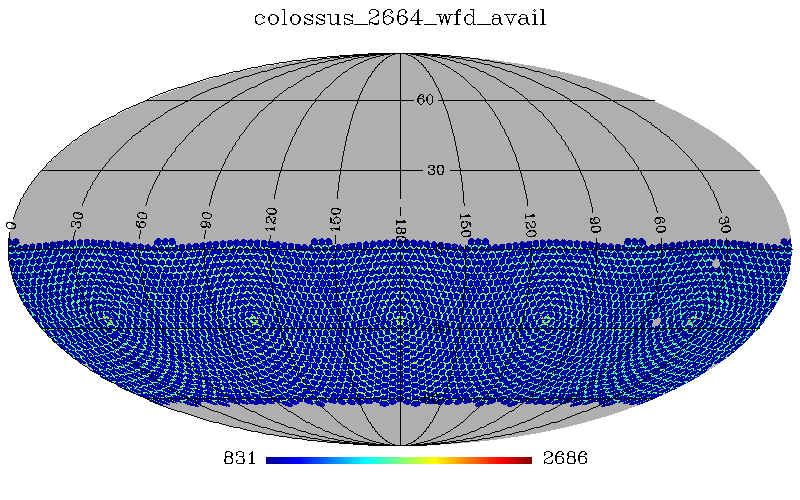
\includegraphics[width=7.0cm]{colossus_2664_wfd_avail_ldep.png} & 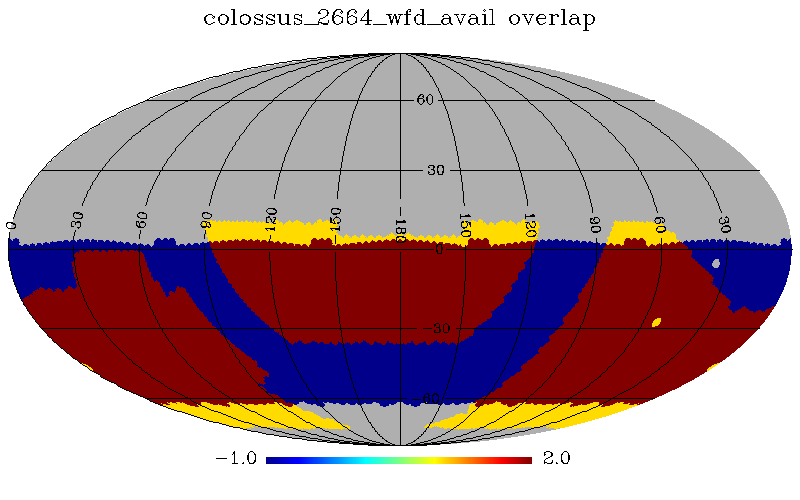
\includegraphics[width=7.0cm]{colossus_2664_wfd_avail_overlap.png} \cr
    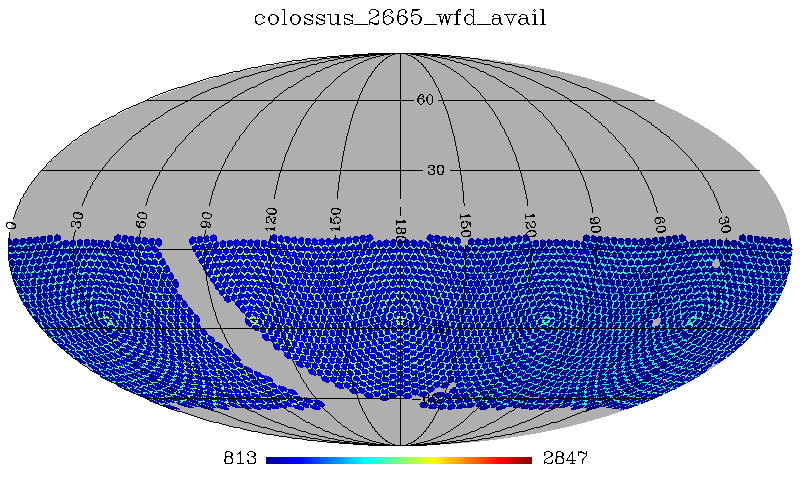
\includegraphics[width=7.0cm]{colossus_2665_wfd_avail_ldep.png} & 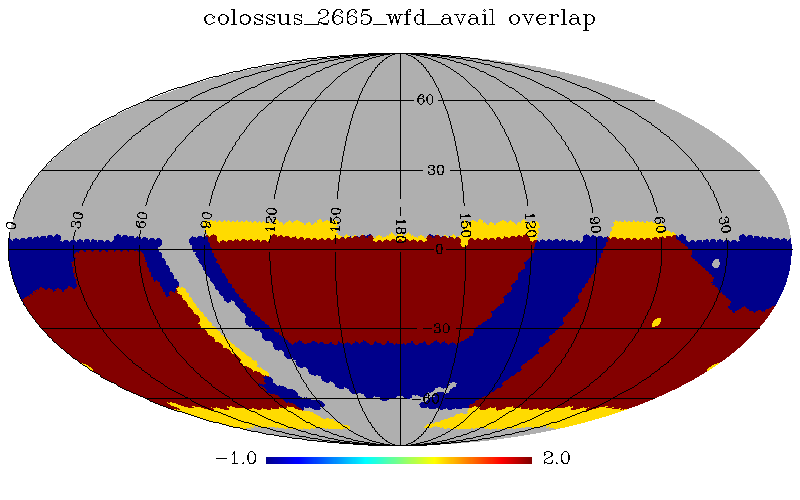
\includegraphics[width=7.0cm]{colossus_2665_wfd_avail_overlap.png} \cr
    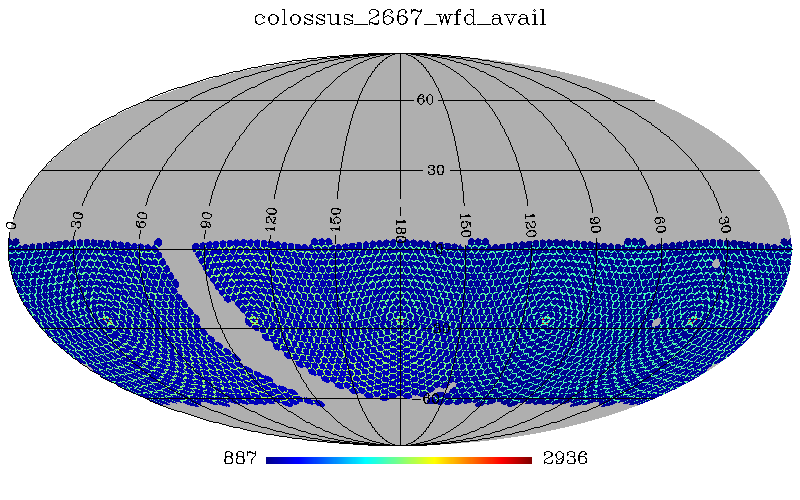
\includegraphics[width=7.0cm]{colossus_2667_wfd_avail_ldep.png} & 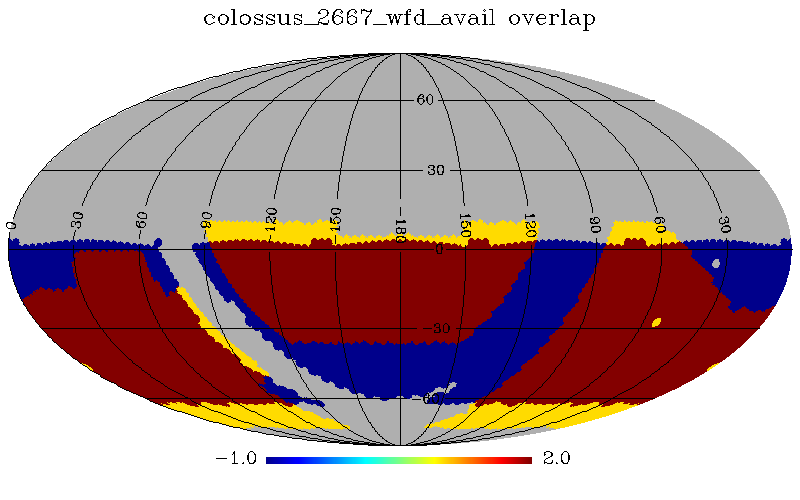
\includegraphics[width=7.0cm]{colossus_2667_wfd_avail_overlap.png} \cr

  \end{tabular}
  \caption{Left: the LSST Healpix maps colour-coded by number of
    visits. Right: The corresponding 4MOST overlap map,
    where red represents the overlap area, blue represents areas of
    LSST WFD that have no 4MOST coverage and yellow represents 4MOST
    area with no LSST coverage. Note that the LSST DDFs are
    deliberately missing from the LSST maps in this analysis. }
  \label{overlap_maps}
\end{figure}

\begin{figure}[htc]
  \begin{tabular}{cc}

    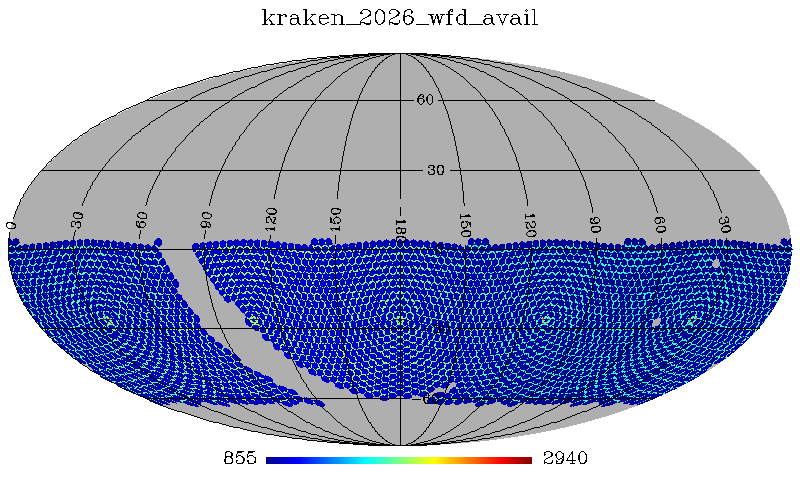
\includegraphics[width=7.0cm]{kraken_2026_wfd_avail_ldep.png} & 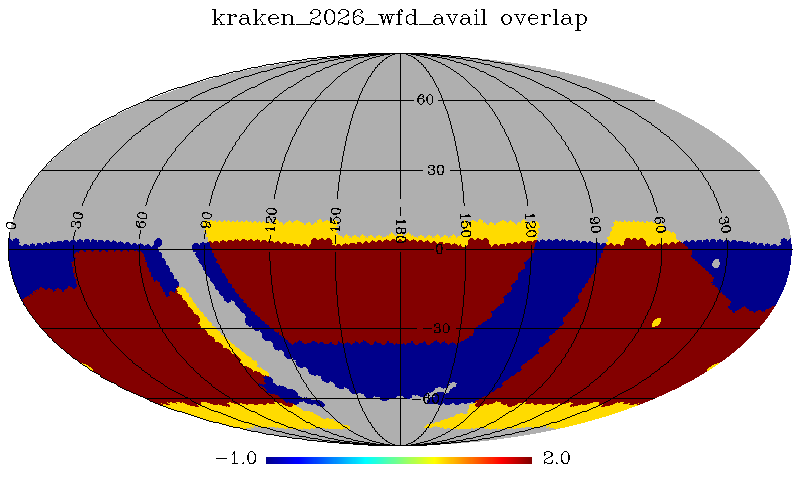
\includegraphics[width=7.0cm]{kraken_2026_wfd_avail_overlap.png} \cr
    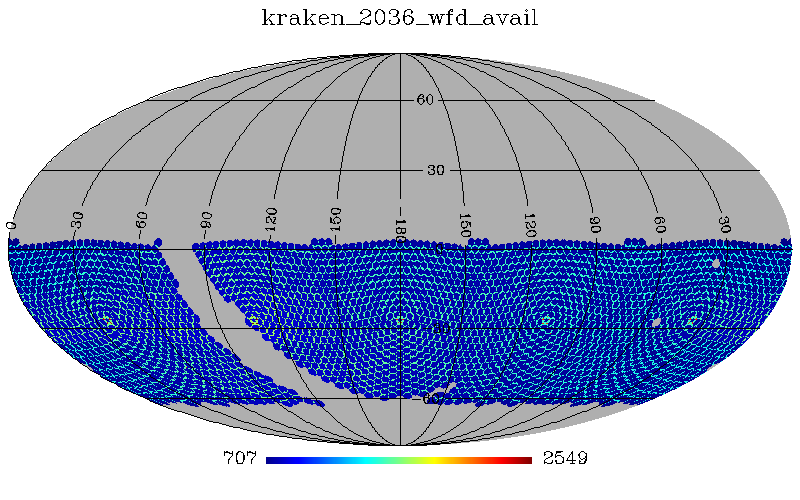
\includegraphics[width=7.0cm]{kraken_2036_wfd_avail_ldep.png} & 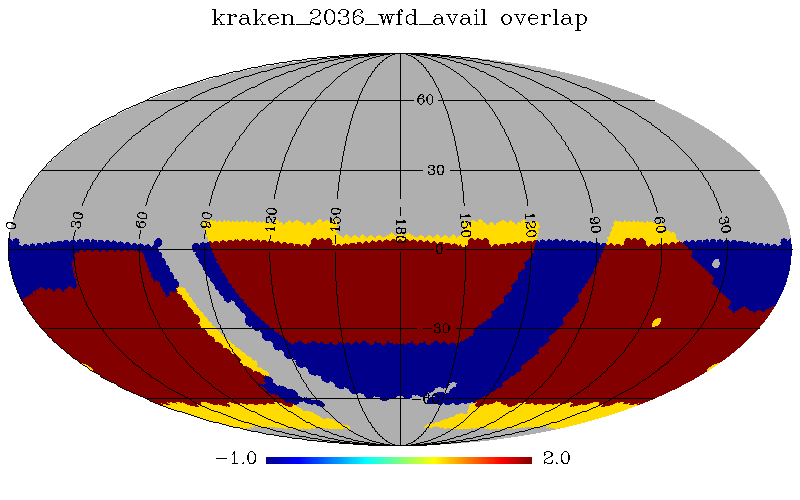
\includegraphics[width=7.0cm]{kraken_2036_wfd_avail_overlap.png} \cr
    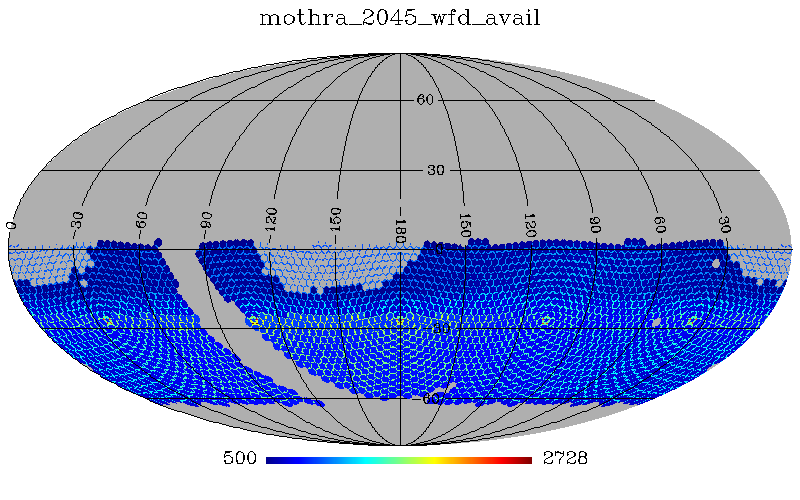
\includegraphics[width=7.0cm]{mothra_2045_wfd_avail_ldep.png} & 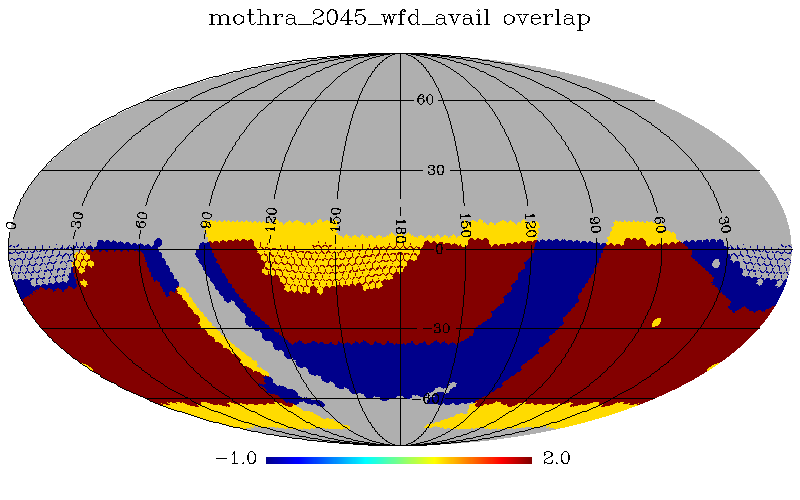
\includegraphics[width=7.0cm]{mothra_2045_wfd_avail_overlap.png} \cr

  \end{tabular}
  \caption{continued}
  
\end{figure}

\begin{figure}[htc]
  \begin{tabular}{cc}
    
    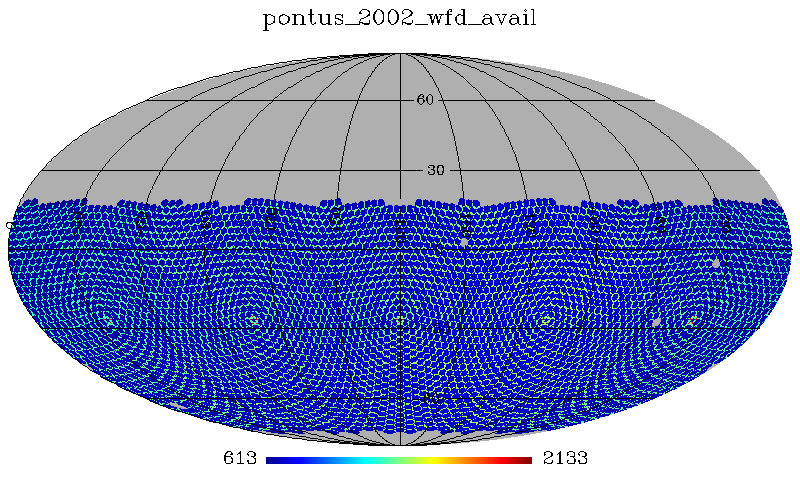
\includegraphics[width=7.0cm]{pontus_2002_wfd_avail_ldep.png} & 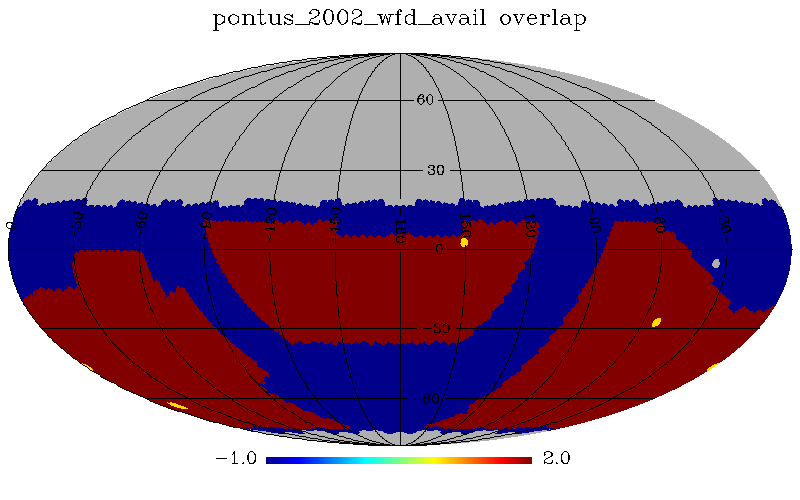
\includegraphics[width=7.0cm]{pontus_2002_wfd_avail_overlap.png} \cr
    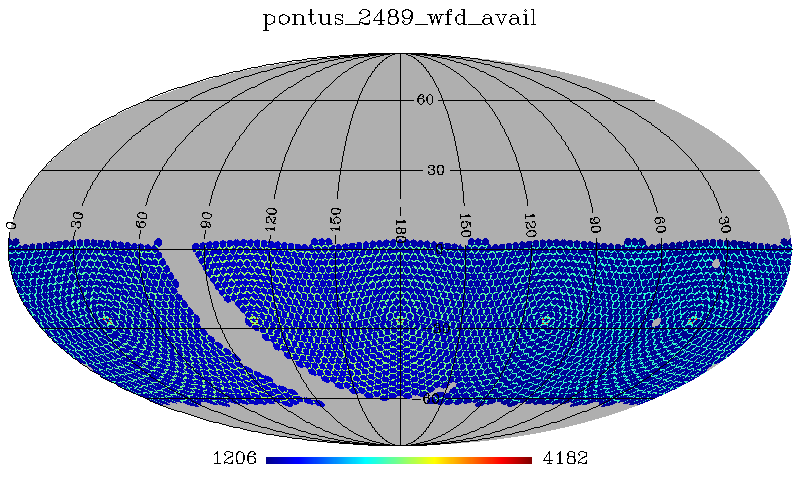
\includegraphics[width=7.0cm]{pontus_2489_wfd_avail_ldep.png} & 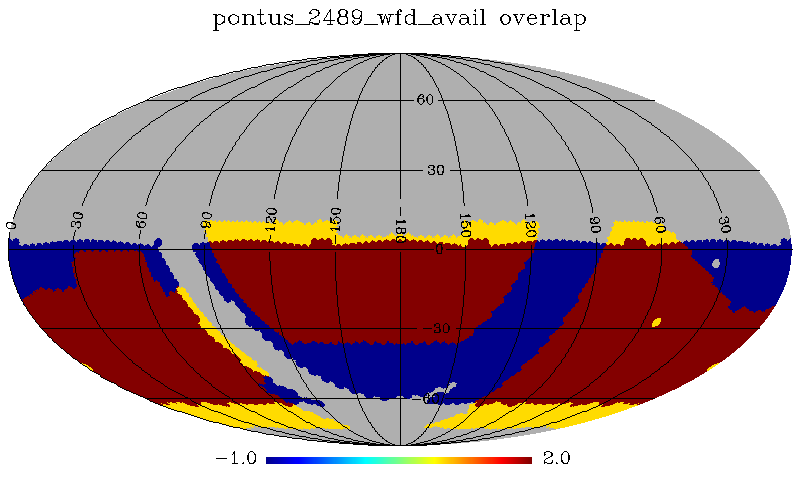
\includegraphics[width=7.0cm]{pontus_2489_wfd_avail_overlap.png} \cr
    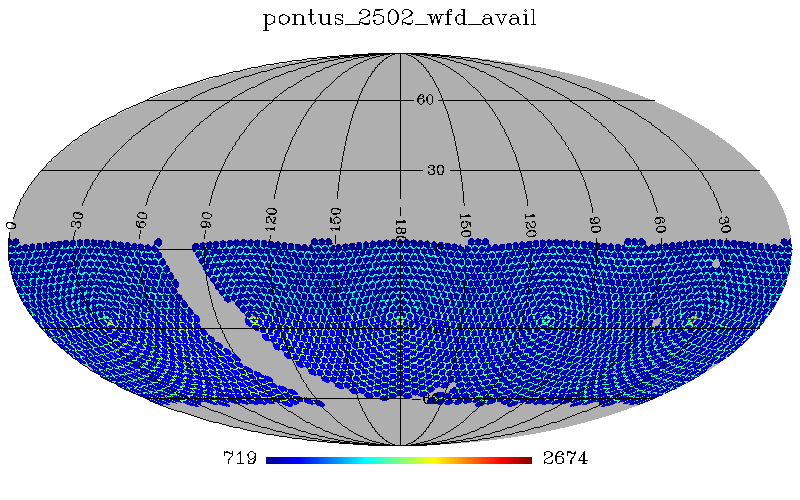
\includegraphics[width=7.0cm]{pontus_2502_wfd_avail_ldep.png} & 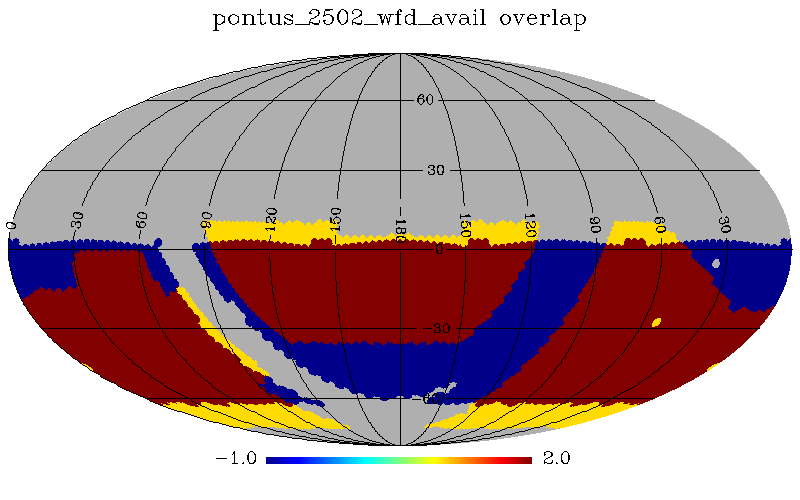
\includegraphics[width=7.0cm]{pontus_2502_wfd_avail_overlap.png} \cr
        
  \end{tabular}
  \caption{continued}
\end{figure}


\subsubsection{Temporal overlap}

4MOST will typically visit each part of the sky twice, for about one
hour exposure ($3\times$ 20 mins) exposures each time (but we
emphasise again that the details of the 4MOST survey are still under
discussion). Clearly, for follow-up of live transients it is important
that 4MOST observes in the areas of sky the LSST has visited recently
(within the lifetime of the transients concerned). For example if LSST
follows a rolling cadence then to maximise trabnsient science, 4MOST
should observe in the same declination range.  Coordination of LSST
and 4MOST surveys is essential.
 	 

\subsubsection{Conclusions}

Of the LSST cadence simulations considered, Pontus\_2002 gives the
largest overall spatial overlap, of approx. 15,000 sq deg, compared to
approximately 12,000-13,000 sq deg for the other surveys. The extended
declination range of Pontus\_2002 increases the overlap with 4MOST,
but goes a little too far in that some of extended LSST area is then
not covered by 4MOST.

As stressed above, temporal coordination of the 4MOST and LSST surveys is
essential if transient science is to me maximised.

\end{document}
